\documentclass[handout]{beamer}
\documentclass{beamer}
\usepackage{amsmath}
\usepackage{graphicx}
\usepackage{xeCJK}
\usepackage{beamerthemeshadow}
\setCJKmainfont{WenQuanYi Zen Hei}
\usetheme{Frankfurt}
%\setbeamercolor{normal text}{bg=yellow!80!green} %background color using xcolor
%\setbeamertemplate{navigation symbols}{}  %no navigation bar
\hypersetup{colorlinks=true,linkcolor=red}
\setbeamertemplate{items}[ball]
\begin{document}
%%-----------------------------------
{
%only show this pic in the titlepage,include it in the {}.
%\setbeamertemplate{background canvas}{
\includegraphics[width=\paperwidth,height=\paperheight]{model.jpg}}
\begin{frame}
    \title{原核基因注释-模型与软件}
    \author{于秋林}
    \institute{结构与功能实验室\\yuqiulin@genomics.cn}
    \maketitle
\end{frame}
}
\newpage
{
\small{                         
\tableofcontents
}
}
%%-------------------------
\section{ORF 确定基因结构}
\begin{frame}[label=ORF]{ORF}
完整的基因结构包含起始密码子和终止密码子:
\begin{itemize}
        \item A genome of length n is comprised of (n/3) codons
        \item Stop codons break genome into segments between consecutive stop codons
        \item The subsegments of these that start from the Start codon (ATG) are ORFs
\end{itemize}
如果序列是随机的,终止密码子应该每21($21=64/3$)个密码子中出现一次,基因长度要大于此长度。设定合理的阈值确定长ORF即可将随机序列与基因分离。
当确定一段orf后可以结合密码子使用偏倚,motif位点特征等进一步分析确定是否是基因。
\end{frame}

%----------------------
\section{Genemark}
\begin{frame}{Genemark}
Genemark:首先用高分样本训练参数,然后采用5阶Markov模型对序列按照不同的读码框打分确定基因结构。后期使用HMM为真核基因结构建模,对应的版本是:GeneMark-E* 和 GeneMark.hmm-E.\\
开发者:\alert{Georgia Institute of Technology, Atlanta, Georgia, USA.}
\end{frame}

\begin{frame}{tradeoff:acuracy vs. feasibility vs. overfit}
在一定范围内,马氏链的阶数越高越好,但通常不会高于10,原因:
\begin{itemize}[<+->]
        \item 计算复杂度,这些串的概率都是用常量存储的,数量是随阶数指数增长的 
        \item 太长的motif会导致支持数据不够 H.influenzae genome size 1.8mb,5-order,$average fold=1.8^6/4^(5+1)=439$ (顺便统计一下每种motif的真实含量,搞清楚那个卡方阈值400到底怎么来的,肯定先从经验分布下手,那个95置信区间是不是虚的?)
\end{itemize}   
\end{frame}

%-----------------------------
%-----------------------------
\section{Glimmer}
\begin{frame}{Glimmer}
Glimmer在定阶马尔科夫模型上做改进,提出可变阶的Interpolated Markov Model。企图利用不同长度的motif更精细地描述数据集特征。\\                                                             
IMM对训练集中不同强度模式充分利用,优先使用强的long motif,如果long motif没有足够的数据支持,IMM 对该long motif 的次阶子串进行打分,并通过一种准确的加权策略利用次阶子串'插值‘出这个long motif分数\alert{(I=interpolated)},如果次级子串仍然没有足够的支持,这种’插值‘还可以继续下去,直到子串短到可以被足够数据支持为止,最短即是单个字符。\\
\end{frame}

\begin{frame}{Glimmer}
Glimmer 的打分策略设计非常巧妙,细节见:
\hyperlink{IMM frame}{\beamerbutton{IMM frame}}\\
% link to the frame 'IMM frame'
1997年的文章:
\alert{Microbial gene identification using interpolated Markov models}\\
1999年的文章:
\alert{Improved microbial gene identification with Glimmer}\\
真核预测的版本:
\alert{http://www.cbcb.umd.edu/software/GlimmerHMM/},同样利用HMM对基因结构建模。\\
\end{frame}
%----------------------------
\section{HMM 模型}
\subsection{生物背景}
\begin{frame}{基因结构可做状态划分}
\begin{figure}
\centering
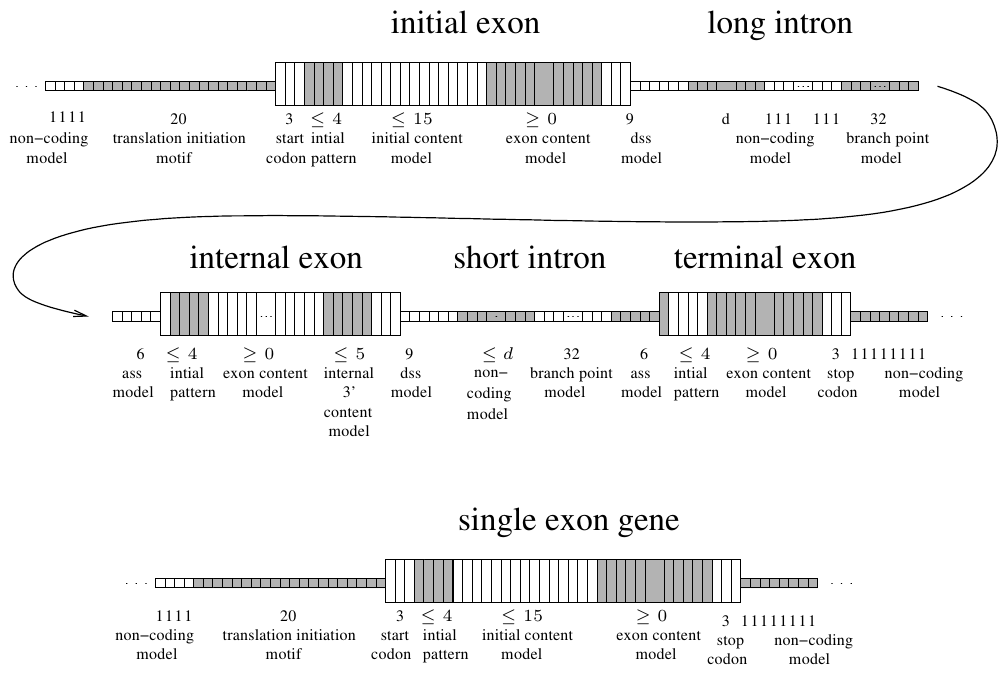
\includegraphics[width=8cm]{../pic/gene-structure.png}
\end{figure}
\end{frame}

%------------------------------
\subsection{HMM in augustus}
\begin{frame}{HMM in augustus}
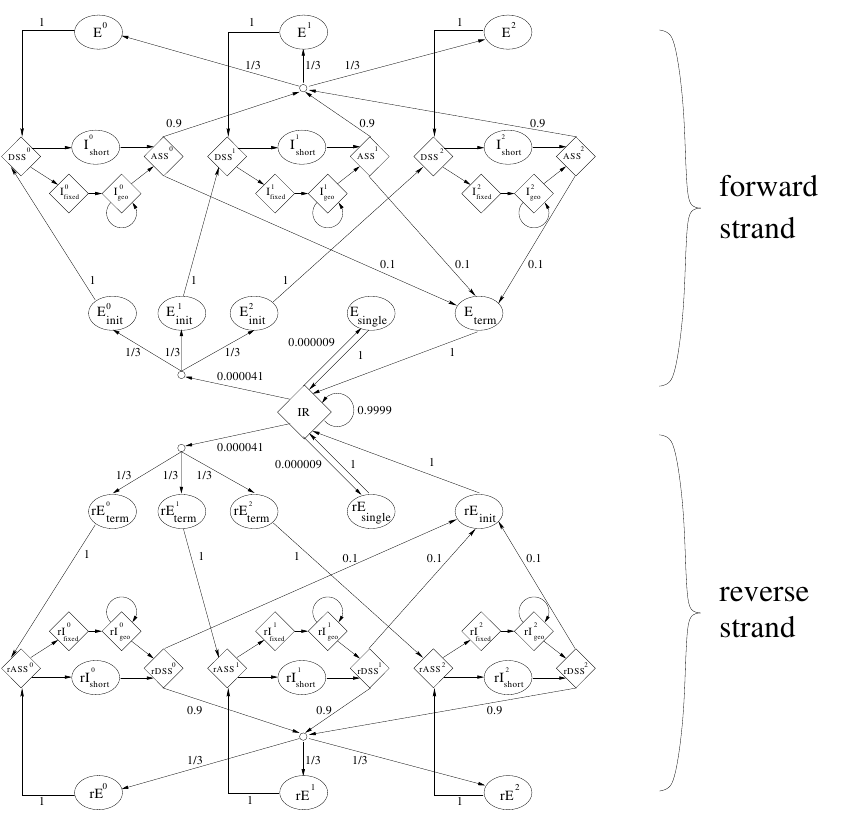
\includegraphics[height=10cm]{../pic/big-scheme.png}
\end{frame}

%------------------------------------
\subsection{外显子建模}
\begin{frame}{外显子建模}
\begin{figure}
\centering
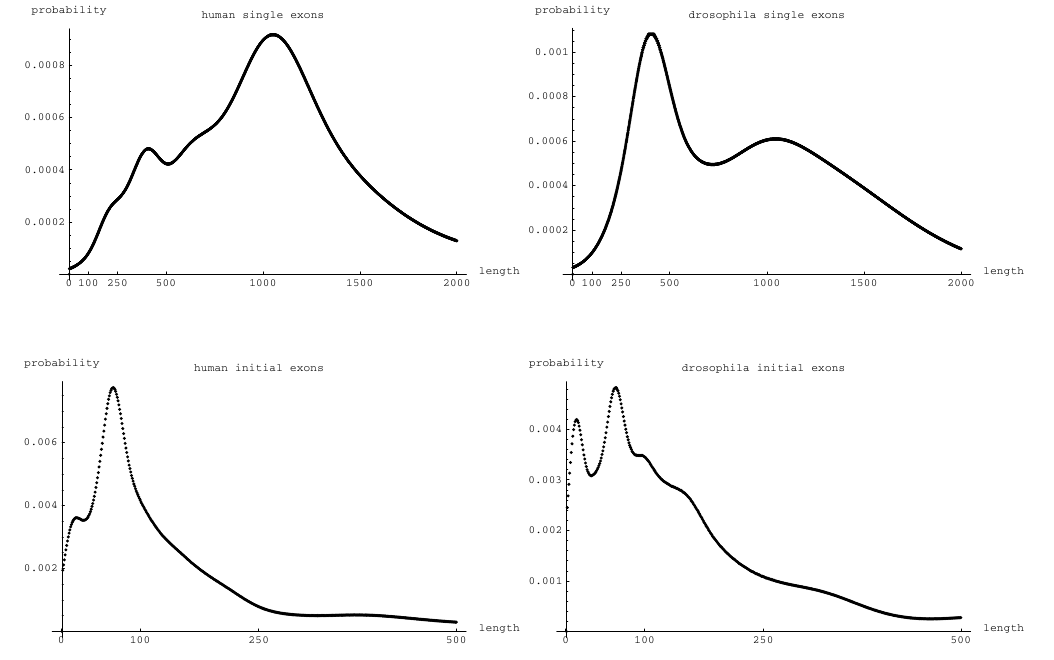
\includegraphics[width=10cm]{../pic/extron-length-1}
\caption{single and initial extron length distribution}
\end{figure}
\end{frame}

\begin{frame}{外显子建模}
\begin{figure}
\centering
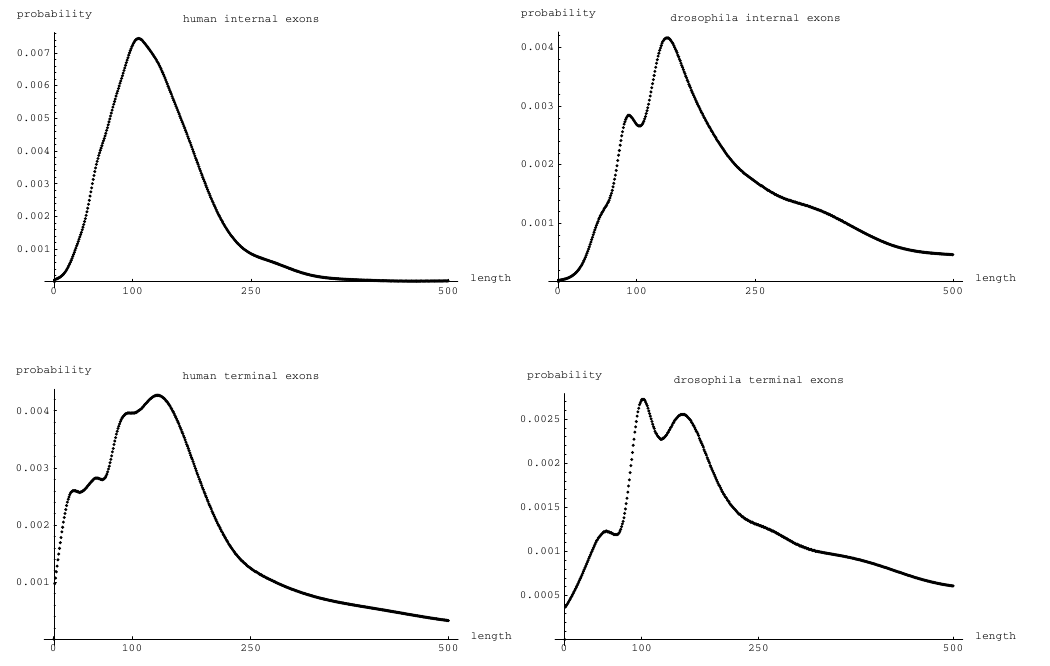
\includegraphics[width=10cm]{../pic/extron-length-2}
\caption{internal and terminal extron length distribution}
\end{figure}
\end{frame}

\begin{frame}{外显子建模}
\begin{itemize}
        \item  human: single, initial, internal, terminal:
        n = 462, n = 822, n = 4334, n = 822, respectively;
        \item Drosophila: single, initial, internal,
        terminal: n = 76, n = 324, n = 917, n = 324, respectively.
        \item 外显子分布窄,可以构造经验分布
        \item 密度估计利用高斯核函数
\end{itemize}   
\end{frame}
%------------------------------------
\subsection{特征序列 \& 子模型}
\begin{frame}{强短信号}
基因上下游有丰富的特征模体(\alert{motif}),有效识别这些模体可以帮助检测潜在基因区域。\\
除了对外显子(内含子)长度建模外,短模式对基因识别也非常重要。
\begin{figure}
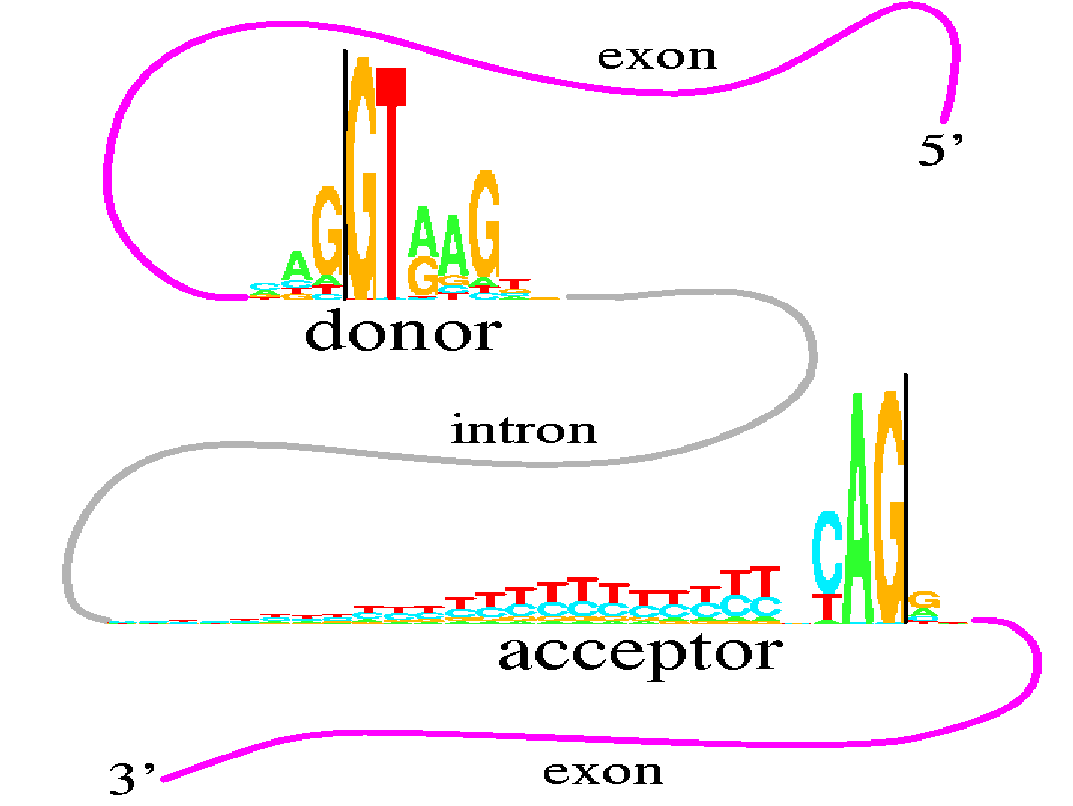
\includegraphics[width=6cm]{../pic/motif_GTAG}
\caption{外显子与内含子之间由GT-AG间隔,这是一个明显的短信号}
\end{figure}

%这是比较强的一个模式: donor 7.9bits,acceptor 9.4bits\\
%注意,所有这些模式都是在可靠比对的maf数据中训练得到的,信息含量的计算同样,仅在训练过程中有用。这些值在预测过程中都是非确定的。
\end{frame}
%-------------------------
\begin{frame}{偏倚数量化}
\begin{figure}
\centering
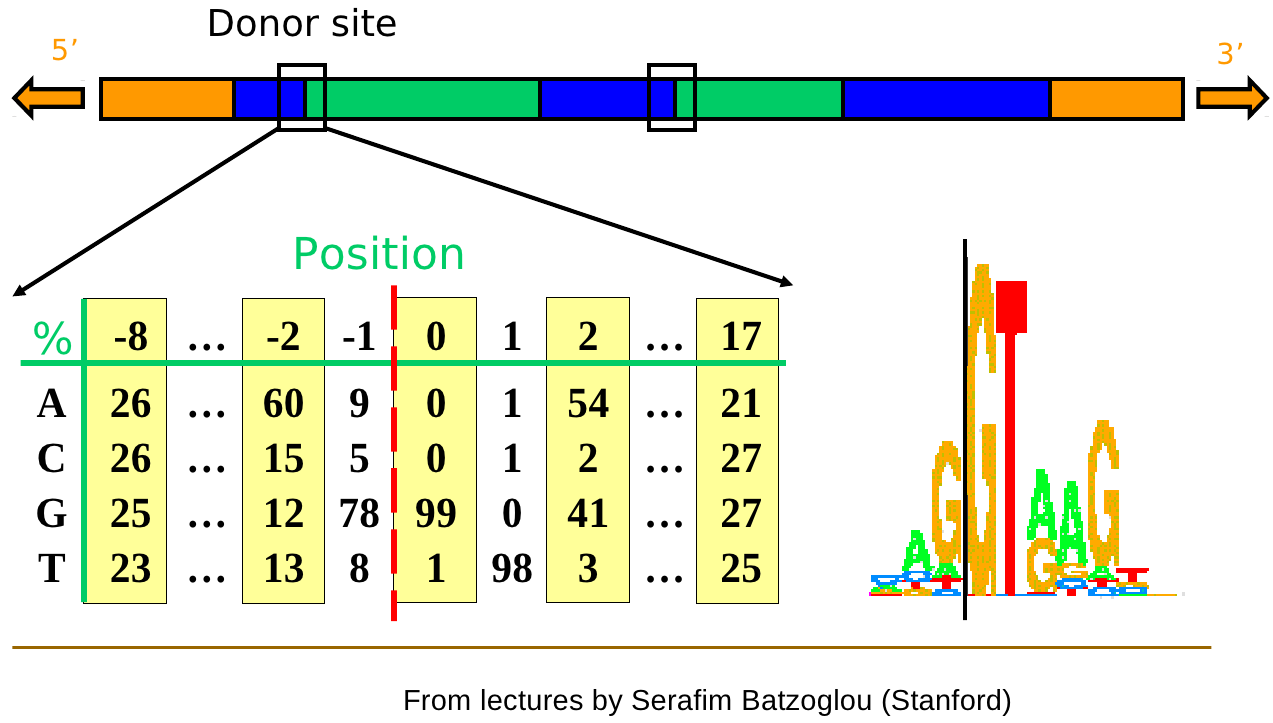
\includegraphics[width=10cm]{../pic/frequency-bias}
\caption{供体位点显示强烈偏倚}
\end{figure}
\end{frame}

\begin{frame}{偏倚数量化}
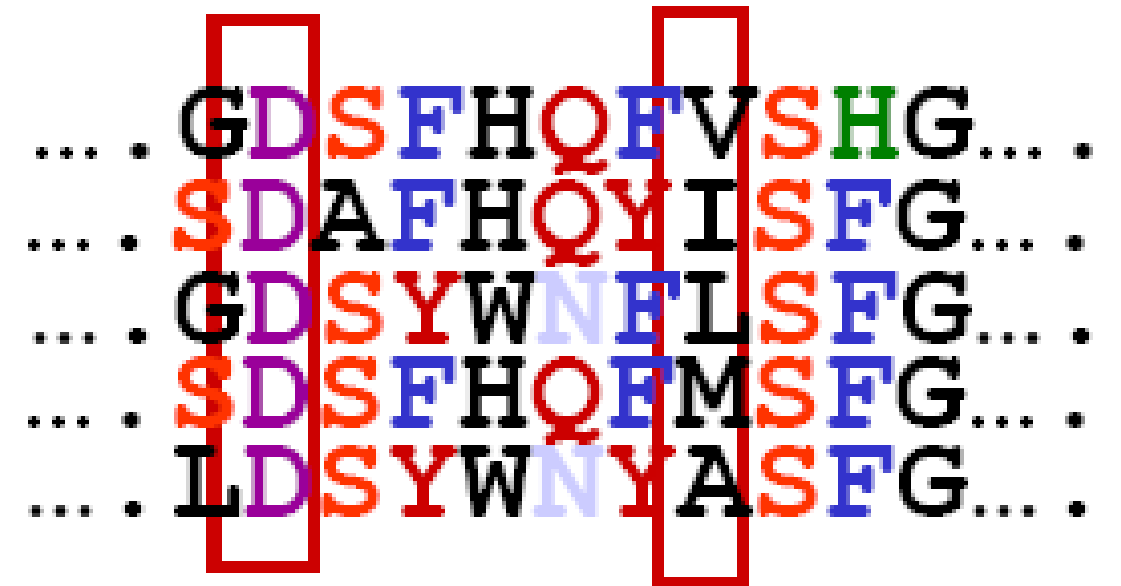
\includegraphics[width=8cm]{../pic/entropy_sample}
\begin{itemize}
\item 位点1:$H_{bg}=-\sum^{20}_{i=1}(1/20)*\log_{2}(1/20)=4.32bit,H_{site1}=0bit$,信号强度:4.32bit\\
\item 位点2:$H_{bg}=-\sum^{20}_{i=1}(1/20)*\log_{2}(1/20)=4.32bit,H_{site2}=4.32bit$,信号强度:0bit
\end{itemize}
\end{frame}
%-----------------------------
%---------------------------
\subsection{利用外部证据推断基因结构}

\begin{frame}{外部证据}
最容易提升性能的部分,除了augustus,genescan等软件也在做这种努力。
\begin{itemize}
\item M manual anchor 
\item P protein database hit
\item E est database hit
\item C combined est/protein database hit
\item D Dialign
\item R retroposed genes
\item T transMapped refSeqs
\end{itemize}   
\end{frame}
%--------------------------------------
\end{document}



